\documentclass[10pt,aps,prb,twocolumn, nofootinbib]{revtex4-1}

\usepackage{amssymb,amsmath}
\usepackage{subfig}
\usepackage{graphicx}
\usepackage{color}
\usepackage{hyperref}
\usepackage{listings}
\usepackage[portuguese]{babel}
\hypersetup{
    bookmarks=true,         % show bookmarks bar?
    unicode=false,          % non-Latin characters in Acrobat’s bookmarks
    pdftoolbar=true,        % show Acrobat’s toolbar?
    pdfmenubar=true,        % show Acrobat’s menu?
    pdffitwindow=false,     % window fit to page when opened
    pdfstartview={FitH},    % fits the width of the page to the window
    pdfauthor={Kevin Multani},     % author
    colorlinks=true,       % false: boxed links; true: colored links
    linkcolor=blue,          % color of internal links
    citecolor=red,        % color of links to bibliography
}
\graphicspath{{figures/}}
\newcommand{\ut}{\ensuremath{\frac{\partial u}{\partial t}}}
\newcommand{\uxx}{\ensuremath{\frac{\partial^2 u}{\partial x^2}}}
\newcommand{\Qt}{\ensuremath{\frac{dQ}{dt}} }
\newcommand{\fixme}{{\bf **FIXME**}}
\renewcommand{\labelitemi}{$\vcenter{\hbox{\tiny$\bullet$}}$}
\begin{document}

\definecolor{dkgreen}{rgb}{0,0.6,0}
\definecolor{gray}{rgb}{0.5,0.5,0.5}
\definecolor{mauve}{rgb}{0.58,0,0.82}

\lstset{frame=tb,
  	language=Matlab,
  	aboveskip=3mm,
  	belowskip=3mm,
  	showstringspaces=false,
  	columns=flexible,
  	basicstyle={\small\ttfamily},
  	numbers=none,
  	numberstyle=\tiny\color{gray},
 	keywordstyle=\color{blue},
	commentstyle=\color{dkgreen},
  	stringstyle=\color{mauve},
  	breaklines=true,
  	breakatwhitespace=true
  	tabsize=3
}

\title{Controle Preditivo baseado em Modelo (MPC) aplicado ao controle de sistemas quânticos}
\author{Gabriel Siqueira Silva, Tales Argolo de Jesus}
\affiliation{Departamento de Computação, Centro Federal de Educação Tecnológica de Minas Gerais, Belo Horizonte, MG, 30510-000 Brasil}

\begin{abstract}

Uma modelagem é proposta para estimar, numericamente, a ação do controle preditivo baseado em modelo, em sistemas quânticos. Comparações entre o método analítico e numerico são apresentadas e demonstram um desvio insignificante fisicamente. As combinações lineares entre dois estados quânticos, produzindo um sistema de dois níveis, são estudados como exemplo. O modelo se torna importante para testes em laboratórios de controle de sistemas dinâmicos visto que a utilização do método analítico é inviável neste meio.

\end{abstract}

\maketitle
\section{\label{sec:one}Introdução}

[\onlinecite{1}].

O nome, Modelo Preditivo de Controle, é proveniente da forma de como a lei de controle é computada. Dado um tempo k, o comportamento do processo através de um horizonte p é considerado. Usando um modelo, a resposta do processo às mudanças na variável manipulada é prevista. Os movimentos das variáveis manipuladas são selecionados de forma que a resposta predita tenha características desejáveis. Apenas a primeira variável manipulada computada é realmente implementada e para o tempo k+1 se repete o processo [\onlinecite{2}].

O MPC pode ser descrito como uma otimização através da manipulação de entradas e do comportamento das previsões do processo. A previsão é realizada com um modelo de processo e portanto é um elemento de um controlador MPC. Modelos não são perfeitos em sua previsão e feedbacks podem melhorar alguns efeitos produzidos por estes [\onlinecite{3}]. 

The goal of this paper is to elucidate the contributions of the three fundamental modes of heat transfer within an end-heated aluminum rod system. Each contribution, \textit{conduction}, \textit{convection}, and \textit{radiation}, is characterized by a physical property of the aluminum rod (heat transport parameters): $\kappa$, $h_c$, $\epsilon$, respectively. Where, $\kappa$ is the thermal conductivity, $h_c$ is the convective coefficient of the system, and $\epsilon$ is the emissivity. The thermal contact resistance between the end heat-source, $R_{th}$ and the specific heat capacity, $c_{Al}$ is also discussed. 
 
Section~\ref{sec:one} delivers a basic mathematical introduction to heat flow theory and provides insight into how the heat transport mechanisms for an end-heated aluminum rod are coupled. Section~\ref{sec:two} describes the experimental setup for all the experiments conducted and assumptions made for each one. Section~\ref{sec:three} presents the results of the experimentation and provides the experimentally determined values for the heat transport parameters, $c_{Al}$, and $R_{th}$ with experimental errors in mind. Section~\ref{sec:four} provides a conclusion with future considerations for further and more accurate experimentation.

\section{\label{sec:one}Theoretical Framework}
The fundamental modes of heat transport in an aluminum rod can be characterized by a parabolic partial differential equation, the \emph{heat equation},

\begin{equation}
\label{eq:one}
\ut - \alpha \uxx + \beta (u-u_{air}) + \gamma (u^4 - u_{air}^4)  = 0.
\end{equation} 
Where $\alpha = \frac{\kappa}{\rho c_{Al}}$, $\rho$ is the density of aluminum, $\beta = \frac{2h_c(L+r)}{\rho c_{Al} r}$, $r$ is the radius of the aluminum rod, $L$ is the total length of the rod, and $\gamma = \frac{2\epsilon \sigma(L+r)}{\rho c_{Al} r}$, $\sigma$ is the Stefan-Boltzmann constant, which is assumed in this paper to be, $\sigma = 5.670373 \times 10^{-8} \text{ W}\text{m}^{-2}\text{K}^{-4}$. Equation~\ref{eq:one} describes the distribution of heat (or variation in temperature) in a given region over time undergoing all three modes of heat transport. For this paper, $u = u(x,t)$ will be the temperature at point, $x$ and time, $t$. 

The solution to equation~\ref{eq:one} (with the proper boundary conditions) fully describes both the transient phase of the effect of heat flow and temperature change and the static (equilibrium) phase of the same. However, analytically solving equation~\ref{eq:one} is difficult. Thus, it is useful to isolate and develop a heat flow model each of the fundamental modes of heat transfer and consider them separately. 

The following discussion of the three modes of heat transport were taken into consideration whilst designing the experiments (see Section~\ref{sec:two}).

\subsection{\label{sec:oneCond}Conduction}
Isolating conduction greatly reduces the complexity of equation~\ref{eq:one}, since the convection and radiation terms are removed, \begin{equation}
\label{eq:two}
\ut - \alpha\uxx = 0.
\end{equation}
Equation~\ref{eq:two} describes the time and spacial evolution of temperature in the aluminum rod subjected to certain boundary conditions. During experimentation, the end of the rod is heated with a constant power source which is delivering heat energy. Since the amount of heat energy per unit time, \Qt is known, it is convenient to view conduction in the following form,
\begin{equation}
\label{eq:three}
\Qt = -\kappa A_{\times}\frac{du}{dx}.
\end{equation}
Where $A_{\times}$ is the cross sectional area. Equation~\ref{eq:three} describes the amount of heat energy transported between two points on the rod. Note it is now clear to see that the unit of $\kappa$ is $\text{W}\text{m}^{-1}\text{K}^{-1}$. The negative sign is indicative of the direction of heat transfer. For simulations, the discrete form of equation~\ref{eq:three} is used (see Appendix~\ref{sec:Aone}). The relationship between equation~\ref{eq:two} and \ref{eq:three} is given by the specific heat equation,

\begin{equation}
\label{eq:four}
\frac{dQ_{net}}{dt} = (c_{Al}\rho dV) u_{rise}.
\end{equation}
Where $\frac{dQ_{net}}{dt}$ is the \emph{net} heat transfer through an infinitesimal volume segment of the rod, and $u_{rise}$ is the corresponding temperature increase of that point. So, using \ref{eq:three} and \ref{eq:four} one can derive \ref{eq:two}.

Furthermore, there exists a finite contact thermal resistance between the heat-power source and the aluminum rod. Using the discrete form of equation~\ref{eq:three}, the absolute thermal resistance between multi-layered contact systems can be determined with,
\begin{equation}
\label{eq:five}
\frac{\Delta Q}{\Delta t} = -\frac{(u_1 - u_2)}{\frac{\frac{\Delta x_1}{\kappa_1} + \frac{\Delta x_2}{\kappa_2} + \dots + \frac{\Delta x_n}{\kappa_n}}{A_{\times}}} = -\frac{\Delta u}{R_{th}}.
\end{equation}
Where $\Delta x_i, \kappa_i$ are the length and conductivities of the multiple layers between the heat source and end of the aluminum rod. Practically, to determine $R_{th}$, a parameter $P_{in}$ is introduced, which is the amount of heat flow that is going through the rod. 
 

\subsection{\label{sec:oneConv}Convection}
Considering convection separately equation~\ref{eq:one} becomes,

\begin{equation}
\label{eq:six}
\ut = -\beta(u-u_{air}).
\end{equation}
Equation~\ref{eq:six} describes the change in temperature due to a differential in the rod and air temperature. A differential in rod and air temperature facilitates heat exchange. The heat exchange is governed by,

\begin{equation}
\label{eq:seven}
\Qt = h_cA_{\circleddash}(u-u_{air}),
\end{equation}
and one can derive  equation~\ref{eq:six} with equation~\ref{eq:seven} by relating them by equation~\ref{eq:four}.  
In equation~\ref{eq:seven}, $A_{\circleddash}$ is the surface area of convection. Also, the units of $h_c$ can be seen to be, $\text{W}\text{m}^{-2}\text{K}^{-1}$. It is important to note that equation~\ref{eq:seven} is a simplification of convective heat flow. The convective coefficient, $h_c$ has geometrical and temperature dependence, but for the purposes of this paper the temperature dependence is neglected. For situations in which the rod is vertical, compared to when the rod is horizontal, the values of $h_c$ differ. This geometrical dependence; the fact that hot air is less dense than cold air, so the rising of hot air in the two different situations (and anything in between) are different, which effects the value of $h_c$. 

Furthermore, one can see that equation~\ref{eq:six} simplifies to an ordinary differential equation\footnote{Convection cooling and heating is sometimes called Newton's Law of Cooling and Heating, in cases where the heat transfer coefficient is independent or relatively independent of the temperature difference between object and environment.}. The solutions to equation \ref{eq:six} are in the form,

\begin{equation}
\label{eq:eight}
u(t) = u_{air} + (u_0 - u_{air})\mathrm{e}^{-\beta t}.
\end{equation}
Where $u_0$ is the initial temperature of the aluminum rod.


\subsection{\label{sec:oneRad}Radiation}
Lastly, isolating the effects of radiation equation~\ref{eq:one} becomes,

\begin{equation}
\label{eq:nine}
\ut = -\gamma(u^4 - u_{air}^4).
\end{equation}
Similar to the convection case, equation~\ref{eq:one} reduces to an ordinary differential equation, equation~\ref{eq:nine}. Furthermore, equation~\ref{eq:nine} may be solved explicitly, using integration techniques. However, the solution is not useful for the purposes of this paper, so it will be left as an exercise for the reader. Rather, the heat transfer relation is more convenient to consider,

\begin{equation}
\label{eq:ten}
\Qt = \epsilon \sigma A_{\circledcirc}(u^4 - u_{air}^4)
\end{equation}
Where $A_{\circledcirc}$ is the surface area of radiation\footnote{For a horizontal cylindrical rod, $A_{\circledcirc} = A_{\circleddash}.$ In other words, the surface area of convection is the same as the surface are of radiation for a bare aluminum rod.} and the unit of $\epsilon$ is $1$, in other words, $\epsilon$ is dimensionless. Equation~\ref{eq:ten} describes the heat transfer via radiation between the surrounding air and the rod. Finally, one is able to derive equation~\ref{eq:nine} using equations~\ref{eq:four} and~\ref{eq:ten}. 

\section{\label{sec:two} Experimental Setup}

Five different experiments were conducted to determine the heat transport parameters. The primary materials used over the course of the experiments were:
	\begin{itemize}\parskip0pt
    	\item $0.3048$ m, $22.5$ mm diameter, $0.327$ kg sand-blasted aluminum rod
        \item $15$ $\Omega$ LTO100 power resistor (heat power source)
        \item $4$ thermocouples (type-T)
        \item Arduino Uno Microcontroller 
        \item DC adjustable power supply
        \item TMP35 room temperature sensor
        \item Tube insulation
        \item Black spray paint
        \item $500$ ml beaker, water and ice
        \item Circuit breadboard and INA2126 instrumentation amplifiers
        \item Stand with rubberized clamps
        \item String
        \item Tgrease 2500 Series Thermal Grease
    \end{itemize}
    
In preparation for all experiments, circuits to amplify the calibrated thermocouple readings and software code for MATLAB-Arduino integration were established.
The experiments conducted are summarized in Table~\ref{tab:experiments}. 

\begin{table}[h]
\caption{\label{tab:experiments}Experiment number and the corresponding heat transfer parameters to be found.}
\scriptsize
\begin{ruledtabular}
\begin{tabular}{cll}
Experiment number & Type of experiment & Parameters from fit\\ \hline
1 & pure conduction & $\kappa$, $ c_{Al}$, $P_{in}$\\ \hline
2 & \begin{tabular}[c]{@{}l@{}}convection\\ bare rod\end{tabular} & $h_c$,  $c_{Al}$, $\epsilon$\\ \hline 
3 & \begin{tabular}[c]{@{}l@{}}coupled conduction\\ and convection\\ bare rod\end{tabular} & $\kappa$, $ c_{Al}$, $h_c$, $\epsilon$, $P_{in}$\\ \hline
4 & \begin{tabular}[c]{@{}l@{}}convection\\ black rod\end{tabular} & $h_c$, $c_{Al}$, $\epsilon$\\ \hline
5 & \begin{tabular}[c]{@{}l@{}}coupled conduction\\ and convection\\ black rod\end{tabular} & $\kappa$, $ c_{Al}$, $h_c$, $\epsilon$, $P_{in}$\\ 
\end{tabular}
\end{ruledtabular}
\end{table}

\bigskip

\subsubsection{\label{sec:twoCond}Pure conduction}
The following experiment was designed based upon the theory discussed in Section~\ref{sec:oneCond} and was carried out to determine the contribution of conduction.

In this experiment, $0.225$ m length of insulation was wrapped around the aluminum rod to minimize the effect of convection and radiation. The rod was held vertically on a stand and the in which the clamp held the insulation. The heat source was attached to one end via nut and bolt. The operating power for the heat source was $10.42$ W. Thermal paste was applied to the contact face of the heat source and the rod to increase thermal conductance. Setting the origin at the end of the rod with the heat source, four calibrated Type-T thermocouples were attached at $x=0$, $x=7.5 \text{ cm}$, $x=15 \text{ cm}$, and $x=22.5 \text{ cm}$. Small holes were drilled in the rod, which the thermocouples were placed in. To ensure that the contact of the thermocouples with the rod was maximized, thermal paste was applied. In order to produce a secure attachment, zip-ties were used.

Furthermore, on the opposite end of the heat source, a portion of the rod was placed into a beaker filled with ice and water. Effectively, this setup kept that boundary at $\approx 0^\circ$, since any excess heat flow from the boundary would go into melting the ice. Note that the effective length of the rod is reduced to $0.225 \text{ m}$ since $x=0.225 \text{ m}\to x=0.3048 \text{ m }$ of the rod was inside of the ice-water beaker ensemble.

The results of the above experiment facilitated the values of thermal conductivity, $\kappa$ and the specific heat capacity of aluminum, $c_{Al}$ and, $P_{in}$ to be known. 

\bigskip 
\noindent $\underline{Assumptions:}$

\begin{itemize}\parskip0pt
    	\item Insulation made it possible to neglect convection and radiation.
    	\medskip
    	\item The end opposite to the heat source stayed at $0^\circ$.
    	\medskip
    	\item Thermocouple calibration was accurate and precise up to experimental limitations.
    	\medskip
    	\item Thermocouple contact was perfect. In other words, the temperature read by the thermocouple was the temperature of the aluminum bar.
    	\medskip
    	\item $\kappa$ was not temperature dependent.
\end{itemize} 

\subsubsection{\label{sec:twoConvbare}Convection with bare rod}
The design of this experiment was based upon the theory discussed in Sections~\ref{sec:oneConv} and \ref{sec:oneRad}. This experiment was conducted to determine the coupling effects of convection and radiation.

A horizontal geometry was chosen for this experiment. So the convective constant, $h_c$ corresponds to a system with cylindrical symmetry. A horizontal geometry was chosen due to the unambiguity of the surface area of convection, $A_{\circleddash}$ and the surface area of radiation, $A_{\circledcirc}$. In fact, in this case, $A_{\circleddash} = A_{\circledcirc}$. Additionally, if a vertical geometry were chosen, then whether the convective parameter of the system would remain constant along the length of the rod would be ambiguous. A non-constant convective parameter would add another degree of complexity to the experiment.

Two sub-experiments were carried out for convection: \textit{Experiment A} and \textit{Experiment B}. In Experiment A, the rod was left to heat from $\approx 0^\circ$ to room temperature, and in Experiment B the rod was left to cool from some temperature above room temperature to room temperature. The reason these two experiments were carried out was to determine if $h_c$ depends on the direction of convective heat flow. Note that the heat source is not attached to the bar in both of the experiments.

\begin{description}
\item[Experiment A] As previously mentioned, the bar was set up with horizontal geometry, in other words, the bar was parallel with the bench top. In order to conduct this experiment, first the bar was fully submerged in a box of ice, the thermocouples attached in the same manner as in Section~\ref{sec:twoCond}. It is imperative that the bar be surrounded by ice on all sides. If the bar is surrounded by ice, only then can it reach a uniform temperature near $\approx 0^\circ$, which will render heat flow via conduction negligible. After enough time had passed for the bar to reach equilibrium ($\approx 45$ minutes) and a uniform temperature distribution, it was taken out and hung from stands with arms via strings and allowed to naturally convect and radiate. 
\end{description}
The results of Experiment A allowed the values of the convective coefficient of the system, $h_c$, the specific heat capacity of aluminum, $c_{Al}$ and emissivity of the aluminum rod, $\epsilon$ to be known. 

\pagebreak
\bigskip
 \noindent $\underline{Assumptions:}$
 
 \begin{itemize}\parskip0pt
     	\item $h_c$ was independent of temperature.
     	\medskip
     	\item The aluminum bar began with a uniform temperature distribution of $\approx 0^\circ$.
     	\medskip
     	\item The string had negligible contribution to the heat transport mechanisms.
     	\item Thermocouple calibration was accurate and precise up to experimental limitations.
     	\medskip
     	\item Thermocouple contact was perfect. In other words, the temperature read by the thermocouple was the temperature of the aluminum bar.
 \end{itemize} 

\begin{description}
\item[Experiment B] Similar to Experiment A, the bar is to be set up with horizontal geometry. In order to conduct this experiment, the bar was submerged in boiling water. However, a beaker large enough to fit the entire rod could not be found. So to attempt to bring the bar to a uniform temperature distribution, half of the bar was put in the boiling water until it reached steady state (with the thermocouple attached), then it was flipped so the other half is in the water. When the temperatures of both halves of the rod were approximately the same, the bar was then hung from strings on stands, thus allowing the bar to convect and radiate naturally. 
\end{description}
The results of Experiment B allowed the values of the convective coefficient of the system, $h_c$, the specific heat capacity of aluminum, $c_{Al}$ and emissivity of the aluminum rod, $\epsilon$ to be known. 

\bigskip
 \noindent $\underline{Assumptions:}$
 
 \begin{itemize}\parskip0pt
     	\item $h_c$ was independent of temperature.
     	\medskip
     	\item The aluminum bar indeed began with a uniform temperature distribution.
     	\medskip
     	\item The string had negligible contribution to the heat transport mechanisms.
     	\item Thermocouple calibration was accurate and precise up to experimental limitations.
     	\medskip
     	\item Thermocouple contact was perfect. In other words, the temperature read by the thermocouple was the temperature of the aluminum bar.
 \end{itemize} 

\subsubsection{\label{sec:twoAllbare} Coupled conduction and convection with bare rod}
The following experiment was designed based upon the theory discussed in Sections~\ref{sec:oneCond}, \ref{sec:oneConv}, and \ref{sec:oneRad}. The experiment was conducted to determine how all three fundamental modes of heat transport behave in conjunction.

The setup of the experiment was as follows: the thermocouples and heat source were placed in the same way as the experiment in Section~\ref{sec:twoCond} and the bar was held horizontally (parallel to the bench top) by two stands with rubber clamps. The heat source delivered was set to deliver $5$ W of power and end opposite to the heat source was simply open to the air.

The results of the above experiment allowed the values of thermal conductivity, $\kappa$, the specific heat capacity of aluminum, $c_{Al}$, convective coefficient of the system, $h_c$, emissivity of the aluminum rod, $\epsilon$ and, $P_{in}$ to be known.

\bigskip
 \noindent $\underline{Assumptions:}$
 
 \begin{itemize}\parskip0pt
    	\item No heat transferred between the rubberized clamp and aluminum rod.
    	\medskip
    	\item Thermocouple calibration was accurate and precise up to experimental limitations.
    	\medskip
    	\item Thermocouple contact was perfect. In other words, the temperature read by the thermocouple was the temperature of the aluminum bar.
    	\medskip
 \end{itemize} 

\subsubsection{\label{sec:twoConvblack} Convection with black rod}
The design of this experiment was based upon the theory discussed in Sections~\ref{sec:oneConv} and \ref{sec:oneRad}. This experiment was conducted to determine the coupling effects of convection and radiation. Essentially, the setup, assumptions, and goals of this experiment were identical to the experiment described in Section~\ref{sec:twoConvbare}, except only experiment B was conducted. Moreover, another difference was the rod was spray-painted black to increase its emissivity, in order to see the increase in contribution of radiative heat transfer. Also, an assumption is made that the spray-paint does not change the conductivity, $\kappa$ and convective heat transfer coefficient, $h_c$. Lastly, another assumption was made for this experiment: the black spray paint was uniformly distributed throughout the rod. 

\subsubsection{\label{sec:twoAllblack} Coupled conduction and convection with black rod}
The following experiment was designed based upon the theory discussed in Sections~\ref{sec:oneCond}, \ref{sec:oneConv}, and \ref{sec:oneRad}. The experiment was conducted to determine how all three fundamental modes of heat transport behave in conjunction with one another. The setup, assumptions, and goals of this experiment was identical to the experiment described in Section~\ref{sec:twoAllbare}. The only difference was the rod was spray-painted black to increase its emissivity, in order to see the increase in contribution of radiative heat transfer. Also, an assumption is made that the spray-paint does not change the conductivity, $\kappa$ and convective heat transfer coefficient, $h_c$. Lastly, another assumption was made for this experiment: the black spray paint was uniformly distributed throughout the rod. 

\section{\label{sec:three}Results and Discussion}
\setcounter{subsubsection}{0}
\renewcommand*{\theHsubsubsection}{chX.\the\value{subsubsection}} %to reset subsubsection numbering

For each individual experiment, the raw data collected was compared to a simulation that matched the experiment (see Appendix~\ref{sec:Aone}). The simulation used a finite difference method of solving either equations~\ref{eq:one}, \ref{eq:two}, \ref{eq:six} or \ref{eq:nine}, with the appropriate boundary conditions. Then, using MATLAB, a least-squared fitting technique was carried out in order to determine the parameters in which the simulation best matched the data (see Appendix~\ref{sec:Atwo}). In order to initiate the simulation, initial guesses for the heat transport parameters, $c_{Al}$, and $P_{in}$ were needed. Table~\ref{tab:simparams} summarizes the initial values inputted for the simulation.

\begin{table}[hb]
    \caption{\label{tab:simparams}Simulation parameter values.}
    \centering
    \begin{ruledtabular}
    \begin{tabular}{ccc}
    	Parameter & Value & Source\\ \hline
        Length & $0.3048$ m & Measurement\\
        Diameter & $0.0225$ m & Measurement\\
        Rod segments & $10$ & Parameter Optimization\\
        $T_{room}$ & $20^\circ \text{C}$ & TMP35 sensor\\
        Density & $2709 \text{ kg}\text{m}^{-3}$ & Measurement\\
        $c_{al}$ & $900 \text{ J}\text{kg}^{-1}\text{K}^{-1} $ & see Ref. \onlinecite{1}\\
        $\kappa$ & $205 \text{ W}\text{m}^{-1}\text{K}^{-1}$ & see Ref. \onlinecite{2}\\
        $h_c$ & $10 \text{ W}\text{m}^{-1}\text{K}^{-2}$  & see Ref. \onlinecite{3}\\
        $\epsilon_{bare}$ & 0 & Approximation\\
        $\epsilon_{black}$ & 1 & Approximation\\
        $P_{in}$ & \begin{tabular}[c]{@{}l@{}}varies between\\ experiments \end{tabular} & Approximation\\
    \end{tabular}
    \end{ruledtabular}
    \end{table}


\subsubsection{\label{sec:threeCond}Pure conduction}

Initially, it was found that the temperature of the rod was not reaching the levels predicted by the simulation. To account for the discrepancy in rod temperatures, it was found to be that all the power that the heat source outputted did go into the rod. Insulation was added to the heat source to rectify the discrepancy and bring the measured data closer to the idealized simulation. 

\begin{figure}[h]
\centering
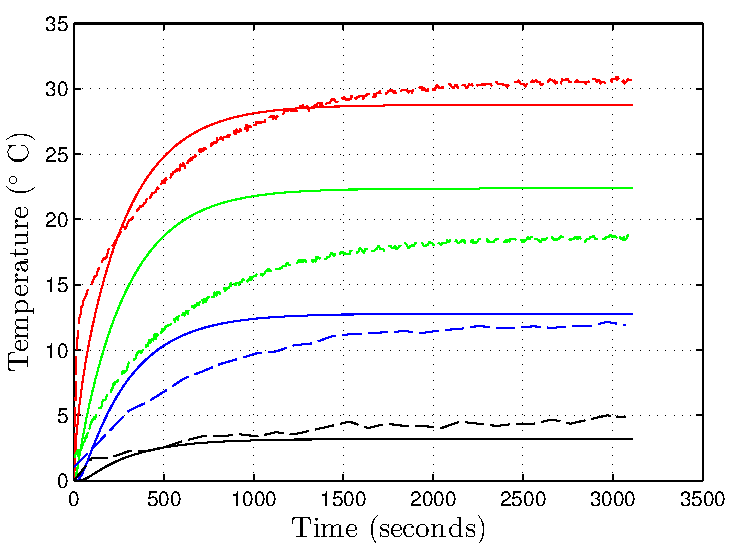
\includegraphics[width=1.0\linewidth]{pureconduction}
\caption{Results of fitted plot to data. Solid lines represent the simulation and dashed lines represent the raw data. {\color{red}\textbf{Red}} corresponds to $x = 0.00$ m, {\color{green}\textbf{green}} to $x = 0.075$ m, {\color{blue}\textbf{blue}} to $x = 0.15$m and \textbf{black} to $x = 0.225$ m. Heat source is located at $x= 0.00$ m, as described in Section~\ref{sec:twoCond}.}
\label{fig:pureconduction}
\end{figure}

Figure~\ref{fig:pureconduction} displays the raw data against the least-squared fitted simulation data. It is important to note that only the thermocouples placed at $x = 0.15$ m and $x = 0.225$ m were used to produce the fitted results. These thermocouples were deemed to be properly calibrated and at a location where no externalities can effect their measurements. However, note that there still exists a discrepancy for the fitted thermocouples against the simulated data. This discrepancy is to be expected as the contact between thermocouples and rod is imperfect and the effect of insulation was not taken into consideration in the simulation. Both of these sources of error imply that the corresponding assumptions made in Section~\ref{sec:twoCond} were incorrect. The remaining two thermocouples had large errors associated with them which can be easily seen on figure~\ref{fig:pureconduction}. The thermocouple located at $x = 0.00$ m measures a temperature higher than the simulation. After careful investigation, this error was deemed to be expected because that thermocouple was placed directly in contact with both the heat source and aluminum rod. This location enables the thermocouple to reach a greater equilibrium temperature than the rod. Furthermore, the thermocouple located at $x = 0.075~\text{ m}$ is completely in disagreement with the simulation. It was deemed that the calibration of this thermocouple was flawed.

 The the simulated fit result in the heat transfer parameters of:
 \begin{center}\fbox{\parbox{0.45\linewidth}{
 	$\kappa = 203.96\text{ W}\text{m}^{-1}\text{K}^{-1}$ \\
 	$c_{Al} =945.31\text{ J}\text{kg}^{-1}\text{K}^{-1}$ \\
 	$P_{in} = 10.37 \text{ W}$}}
 \end{center}
 The average error between the thermocouples and the simulated fit data is $0.1030 ^\circ$C, which is within reasonable experimental uncertainty. Using the $P_{in}$ parameter determined from the fit (see figure~\ref{fig:pureconduction}), equation~\ref{eq:five}, the thermal contact resistance between the heat  [\onlinecite{5}], thermal paste [\onlinecite{6}] and aluminum rod system was, $\boxed{R_{th} = 3.52 \text{ K}\text{W}^{-1}}$.

\subsubsection{\label{threeConv} Convection with bare rod}
The following section will provide results on the two experiments outlined in section~\ref{sec:twoConvbare}.
\newpage
\begin{description}
\item[Experiment A]
\end{description}

As described in Section~\ref{sec:twoConvbare} the entire bar was chilled to a uniform temperature of $\approx 5^\circ \text{C}$ and heated up to a temperature of $\approx 20^\circ \text{C}$. Figure~\ref{fig:bareHeating} displays the raw data against the least squared fitted simulation data. There is only one resultant fit because the theory discussed in section~\ref{sec:oneConv} implies that there is no $x$ dependence on convective heat transfer. From this, it can be concluded that the convective transfer coefficient, $h_c$ is also independent of the location on the rod (for a horizontal geometry).  

\begin{figure}[h]
\centering
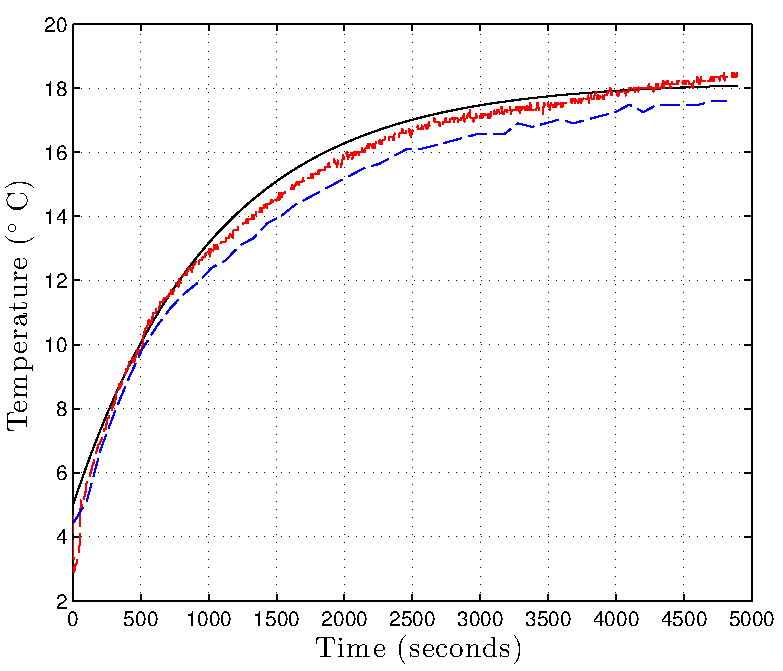
\includegraphics[width=1.0\linewidth]{bareHeating}
\caption{Results of fitted plot to data. Solid \textbf{black} line represents the result from the fitted simulation and dashed lines represent the raw data from the thermocouples. {\color{red}\textbf{Red}} corresponds to $x = 0.00$ m, {\color{blue}\textbf{blue}} to $x = 0.15$ m.}
\label{fig:bareHeating}
\end{figure}
 The the simulated fit result in the heat transfer parameters of:
\begin{center}\fbox{\parbox{0.45\linewidth}{
 	$h_c = 12.00\text{ W}\text{m}^{-2}\text{K}^{-1}$ \\
 	$c_{Al} =925.53\text{ J}\text{kg}^{-1}\text{K}^{-1}$ \\
 	$\epsilon = 0.200 $}}
\end{center}

\noindent The average error between the thermocouples and the simulated fit data is $0.0228 ^\circ$C, which is within reasonable experimental uncertainty. Note, two thermocouples ($x = 0.075 \text{ m}$ and $x = 0.225 \text{ m}$) were ignored as their temperature readings were unreliable due to mis-calibration. This complication does not effect the integrity of the results because it is known from Section~\ref{sec:oneConv} that all the thermocouples should theoretically produce the same curve. 

Furthermore, the thermocouples in figure~\ref{fig:bareHeating} both record a temperature lower than the simulation. This phenomenon can be explained by the fact that the thermocouples may conduct heat from the tip of the measurement probe, therefore producing a measurement for the temperature that is lower than the temperature of the rod. This conclusion leaves the corresponding assumption made for experiment A in Section~\ref{sec:twoConvbare} moot. 

\begin{description}
\item[Experiment B]
\end{description}

As described in Section~\ref{sec:twoConvbare} the entire bar was heated to a uniform temperature of $\approx 55^\circ \text{C}$ and heated up to a temperature of $\approx 20^\circ \text{C}$. Figure~\ref{fig:bareCooling} displays the raw data against the least squared fitted simulation data. There is only one resultant fit because the theory discussed in section~\ref{sec:oneConv} implies that there is no $x$ dependence on convective heat transfer.   

\begin{figure}[h]
\centering
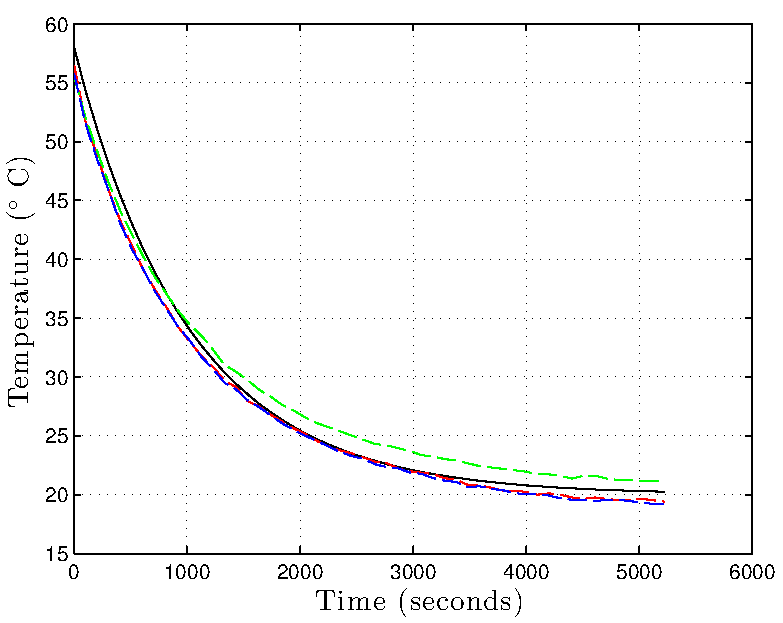
\includegraphics[width=1.0\linewidth]{bareCooling}
\caption{Results of fitted plot to data. Solid \textbf{black} line represents the result from the fitted simulation and dashed lines represent the raw data from the thermocouples. {\color{red}\textbf{Red}} corresponds to $x = 0.00$ m, {\color{green}\textbf{green}} to $x = 0.075$ m, and {\color{blue}\textbf{blue}} to $x = 0.15$ m.}
\label{fig:bareCooling}
\end{figure}
The the simulated fit result in the heat transfer parameters of:
\begin{center}\fbox{\parbox{0.45\linewidth}{
 	$h_c = 11.54\text{ W}\text{m}^{-2}\text{K}^{-1}$ \\
 	$c_{Al} =899.76\text{ J}\text{kg}^{-1}\text{K}^{-1}$ \\
 	$\epsilon = 0.199 $}}
\end{center}

\noindent The average error between the thermocouples and the simulated fit data is $0.0214 ^\circ$C, which is within reasonable experimental uncertainty. Note, one thermocouple ($x = 0.225 \text{ m}$) was ignored as its temperature readings were unreliable due to mis-calibration. This complication does not effect the integrity of the results because it is known from Section~\ref{sec:oneConv} that all the thermocouples should theoretically produce the same curve. 

Furthermore, the thermocouples in figure~\ref{fig:bareHeating} show a minimal amount of discrepancy with respect to the simulation fit. This discrepancy is expected, since the method the bar was heated, explained in Section~\ref{sec:twoConvbare}, is flawed. The method may create a small temperature differential inside the bar, allowing some conduction to occur. This conduction is responsible for the slight discrepancies.

\subsubsection{\label{sec:threeAllbare}Coupled conduction and convection with bare rod}

As described in Section~\ref{sec:twoAllbare}, all three fundamental modes of heat transport were analyzed for a bare rod. Figure~\ref{fig:allThreeBare} displays the raw data against the least squared fitted simulation data. The 

\begin{figure}[h!]
\centering
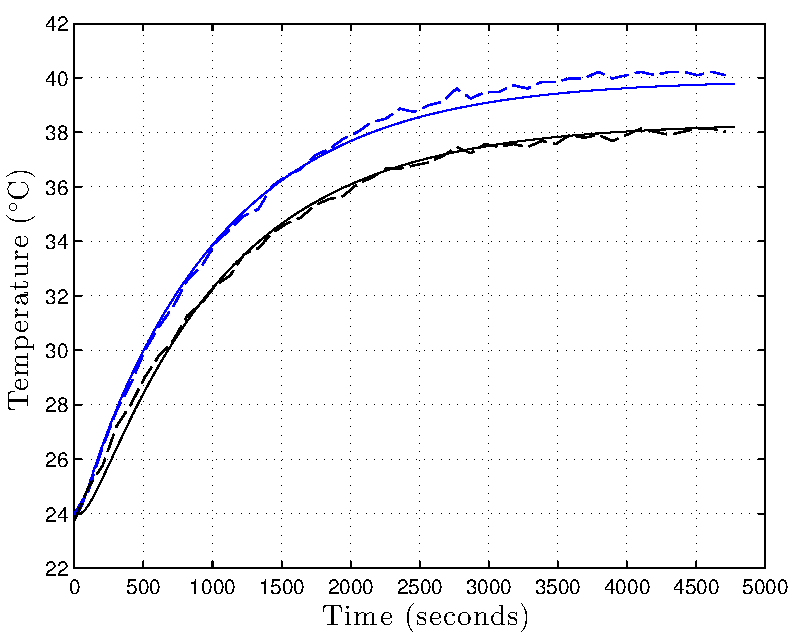
\includegraphics[width=1.0\linewidth]{allThreeBare}
\caption{Results of fitted plot to data. Solid lines represent the simulation and dashed lines represent the raw data. {\color{blue}\textbf{Blue}} to $x = 0.15$m and \textbf{black} to $x = 0.225$ m. Heat source is located at $x= 0.00$ m, as described in Section~\ref{sec:twoAllbare}.}
\label{fig:allThreeBare}
\end{figure}

The fitted simulation yields the physical parameters:
\bigskip
\begin{center}\fbox{\parbox{0.6\linewidth}{
	$\kappa = 185.32\text{ W}\text{m}^{-1}\text{K}^{-1}$ \\
    $h_c = 11.90\text{ W}\text{m}^{-2}\text{K}^{-1}$ \\
	$\epsilon =  0.231$\\
    $c_{Al} = 930.02\text{ J}\text{kg}^{-1}\text{K}^{-1}$ \\
    $P_{in} = 4.998 \text{ W} $
}}
\end{center}
The average error from the simulation lines to the three thermocouple data sets is $0.1036 ^\circ$C, which is within reasonable experimental uncertainty. Two thermocouples ($x = 0.00 \text{ m}$ and $x = 0.075 \text{ m}$) were ignored as their temperature readings were unreliable due to mis-calibration. The impact of two unreliable thermocouples was insignificant. The two reliable thermocouples were enough to generate simulated fit parameters that matched those of previous experiments. Furthermore, figure~\ref{fig:allThreeBare} shows minimal discrepancy and can be accredited to noise.

Using the $P_{in}$ parameter determined from the fit (see figure~\ref{fig:allThreeBare}), equation~\ref{eq:five}, the thermal contact resistance between the heat source [\onlinecite{5}], thermal paste [\onlinecite{6}] and aluminum rod system was, $\boxed{R_{th} = 3.14 \text{ K}\text{W}^{-1}}$.


\subsubsection{\label{sec:threeConvblack} Convection with black rod}
As described in Section~\ref{sec:twoConvblack} the entire bar was heated to a uniform temperature of $\approx 53^\circ \text{C}$ and cooled up to a temperature of $\approx 20^\circ \text{C}$. Figure~\ref{fig:blackCooling} displays the raw data against the least squared fitted simulation data. There is only one resultant fit because the theory discussed in section~\ref{sec:oneConv} implies that there is no $x$ dependence on convective heat transfer.   

\begin{figure}[h]
\centering
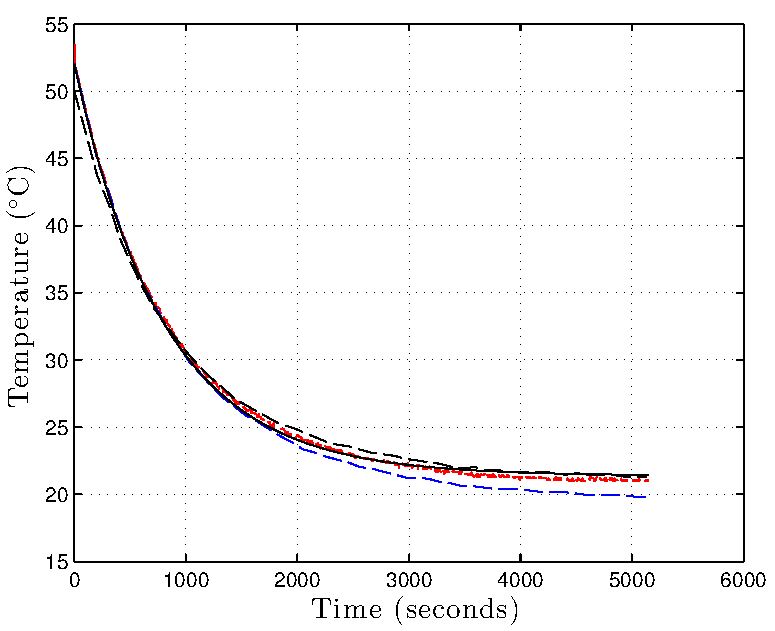
\includegraphics[width=1.0\linewidth]{blackCooling}
\caption{Results of fitted plot to data. Solid \textbf{black} line represents the result from the fitted simulation and dashed lines represent the raw data from the thermocouples. {\color{red}\textbf{Red}} corresponds to $x = 0.00$ m, and {\color{blue}\textbf{blue}} to $x = 0.15$ m.}
\label{fig:blackCooling}
\end{figure}
The the simulated fit result in the heat transfer parameters of:
\begin{center}\fbox{\parbox{0.45\linewidth}{
 	$h_c = 11.94\text{ W}\text{m}^{-2}\text{K}^{-1}$ \\
 	$c_{Al} =985.30\text{ J}\text{kg}^{-1}\text{K}^{-1}$ \\
 	$\epsilon = 0.923 $}}
\end{center}

\noindent The average error between the thermocouples and the simulated fit data is $0.0268 ^\circ$C, which is within reasonable experimental uncertainty. Note, one thermocouple ($x = 0.075 \text{ m}$) was ignored as its temperature readings were unreliable due to mis-calibration. This complication does not effect the integrity of the results because it is known from Section~\ref{sec:oneConv} that all the thermocouples should theoretically produce the same curve. 

Moreover, the thermocouples in figure~\ref{fig:bareHeating} show a minimal amount of discrepancy with respect to the simulation fit. This discrepancy is expected, since the method the bar was heated, explained in Section~\ref{sec:twoConvblack}, is flawed. The method may create a small temperature differential inside the bar, allowing some conduction to occur. This conduction is responsible for the slight discrepancies.

\subsubsection{\label{sec:threeAllblack} Coupled conduction and convection with black rod}

As described in Section~\ref{sec:twoAllblack}, all three fundamental modes of heat transport were analyzed for a black rod. Figure~\ref{fig:allThreeBlack} displays the raw data against the least squared fitted simulation data.

\begin{figure}[h!]
\centering
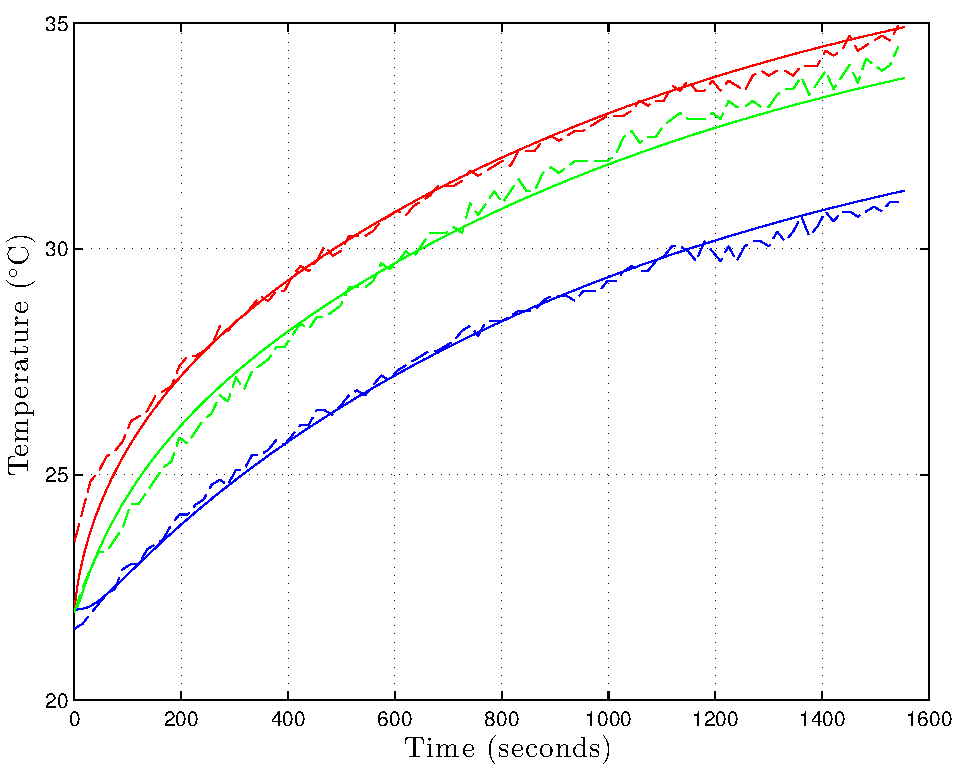
\includegraphics[width=1.0\linewidth]{allThreeblack}
\caption{Results of fitted plot to data. Solid \textbf{black} line represents the result from the fitted simulation and dashed lines represent the raw data from the thermocouples. {\color{red}\textbf{Red}} corresponds to $x = 0.00$ m, {\color{green}\textbf{green}} to $x = 0.075$ m, and {\color{blue}\textbf{blue}} to $x = 0.15$ m. Heat source is located at $x= 0.00$ m, as described in Section~\ref{sec:twoAllblack}.}
\label{fig:allThreeBlack}
\end{figure}

The fitted simulation yields the physical parameters:
\bigskip
\begin{center}\fbox{\parbox{0.6\linewidth}{
	$\kappa = 253.74\text{ W}\text{m}^{-1}\text{K}^{-1}$ \\
    $h_c = 12.74\text{ W}\text{m}^{-2}\text{K}^{-1}$ \\
	$\epsilon =  0.916$\\
    $c_{Al} = 985.44\text{ J}\text{kg}^{-1}\text{K}^{-1}$ \\
    $P_{in} = 4.05 \text{ W} $
}}
\end{center}
The average error from the fitted simulation to the three thermocouples is $0.0219 ^\circ$C, which is within reasonable experimental uncertainty. One thermocouple ($x = 0.225 \text{ m}$) was ignored as its temperature readings were unreliable due to mis-calibration. The impact of the unreliable thermocouple was insignificant. The three reliable thermocouples were enough to generate simulated fit parameters that matched those of previous experiments. Furthermore, figure~\ref{fig:allThreeBlack} shows minimal discrepancy and can be accredited to noise.

Using the $P_{in}$ parameter determined from the fit (see figure~\ref{fig:allThreeBlack}), equation~\ref{eq:five}, the thermal contact resistance between the heat source [\onlinecite{5}], thermal paste [\onlinecite{6}] and aluminum rod system was, $\boxed{R_{th} = 3.85 \text{ K}\text{W}^{-1}}$.

\subsection*{Summary of Results}

Compiling all the results in Section~\ref{sec:three} and determining their inherent, experimental relative errors (table~\ref{tab:summResults}) and with respect to accepted values of the heat transfer parameters, table~\ref{tab:summResults} is established.
\begin{table}[hb]
    \caption{\label{tab:summResults}Summary of all the fitted results and their respective relative errors from the furthest empirically obtained value.}
    \centering
    \begin{ruledtabular}
    \begin{tabular}{cc}
    	Parameter & Value\\ \hline
        $\kappa$ & $214.34 \pm 18.40\% \text{ W}\text{m}^{-1}\text{K}^{-1}$\\
        $h_c$ & $12.02 \pm 6.00 \% \text{ W}\text{m}^{-2}\text{K}^{-1}$ \\
        $\epsilon_{bare}$ & $0.210 \pm 10.00\%$ \\
        $\epsilon_{black}$ & $0.867 \pm 6.46\%$\\
        $c_{Al}$ & $945.23 \pm 4.81\% \text{ J}\text{kg}^{-1}\text{K}^{-1}$ \\
        $R_{th}$ & $3.503 \pm 11 \% \text{ K}\text{W}^{-1} $ \\
    \end{tabular}
    \end{ruledtabular}
\end{table}

\begin{table}[hb]
    \caption{\label{tab:summResultsActual}Summary of all the fitted results and their respective relative errors from the accepted value. See Ref.~\onlinecite{1}, ~\onlinecite{2}, ~\onlinecite{3}, ~\onlinecite{4} for accepted values.}
    \centering
    \begin{ruledtabular}
    \begin{tabular}{ccc}
    	Parameter & Value & Actual Value\\ \hline
        $\kappa$ & $214.34 \pm 4.56\% \text{ W}\text{m}^{-1}\text{K}^{-1}$ &$ 205\text{ W}\text{m}^{-1}\text{K}^{-1}$ \\
        $h_c$ & $12.02 \pm 20.20 \% \text{ W}\text{m}^{-2}\text{K}^{-1}$ & $10 \text{ W}\text{m}^{-2}\text{K}^{-1}$ \\
        $\epsilon_{bare}$ & $0.210 \pm 10.00\%$ & $0.210$  \\
        $\epsilon_{black}$ & $0.867 \pm 6.46\%$ &  $0.867$\\
        $c_{Al}$ & $945.23 \pm 5.03\% \text{ J}\text{kg}^{-1}\text{K}^{-1}$ & $900 \text{ J}\text{kg}^{-1}\text{K}^{-1}$\\
        $R_{th}$ & $3.503\text{ K}\text{W}^{-1} $ \textit{error not applicable} & \textit{not applicable}\\
    \end{tabular}
    \end{ruledtabular}
\end{table}
    
\subsection*{Discussion}
As tables~\ref{tab:summResults} and ~\ref{tab:summResultsActual} depict, there are two different types of errors that one can reason about. Most of these errors were outlined with the results in Section~\ref{sec:three}, as a summary:

\begin{footnotesize}
	\begin{itemize}\parskip0pt
    \item Small errors in thermocouple calibrations propagating through amplifier circuits.
    \item No model of insulation in simulation, which leads to errors in fitting.
    \item Errors in unwanted heat transfer mechanisms. For example, having conduction heat transfer contributions in the pure convection and radiation experiments.
    \item Small errors in thermal resistance can be taken into account by the fact that uneven amounts can be applied (or the same amount is not applied each experiment).
    \item Thermocouples conducting heat from the rod, thus lowering the temperature measurement.
    \item Room temperature fluctuations may cause errors (day and night temperature fluctuations).
    \end{itemize}
\end{footnotesize}

 
\section{\label{sec:four}Conclusion}

Improvements can be made for future experimentation. Possible improvements would include increasing the accuracy of temperature measurements. This improvement would include: higher quality thermocouples and an improved method to secure the thermocouples onto the rod. A more sophisticated modeling process would improve simulation results since it will model the real situation closer than the 1-D approximation done in this paper. Additionally, carrying out the experiment in a more controlled environment would help reduce noise, temperature fluctuations and unwanted non-linear effects from the surroundings. Inside the laboratory, there can be many sources of thermodynamic heat transfer processes occurring such as: movement of humans, air conditioning, pressure, humidity, day and night temperature. If one can control as many of these as possible, a characteristic value for the heat transfer parameters can be better determined.

In closing, the heat transport parameters: thermal conductivity, $\kappa$ , the convective coefficient of the system $h_c$, emissivity of a bare, sand-blasted aluminum rod, $\epsilon_{bare}$ and emissivity of a spray-painted black aluminum rod, $\epsilon_{black}$ were determine, as well as, the specific heat capacity $c_{Al}$ and thermal contact resistance with an LTO100 power resistor, $R_{th}$. These values were obtained in a fairly accurate manner. Finally, the three fundamental modes of heat transport: conduction, convection, and radiation were discussed an analyzed for an aluminum rod.

\appendix
\section{\label{sec:Aone}MATLAB Simulation Code}
The following function takes the parameters of the heat transport mechanisms and generates a simulation of temperature versus time. 
\lstinputlisting{getTemperatureGradient.m}
\newpage
The following function uses the above simulation to generate a position versus time plot for the temperature of the rod at any position, $x$.
\lstinputlisting{getTemperatureVector.m}
\section{\label{sec:Atwo}MATLAB Fitting Code}
The following code utilizes the simulation in Appendix~\ref{sec:Aone} and performs the least squares fitting algorithm to minimize the error between the simulation plot and experimental data, extracting the fitted heat parameter values.
\lstinputlisting{generalFit.m}

\bibliography{bib}

\end{document}